\documentclass{ximera}[font=12pt]  % I don't think font works

\title{Fractions: Prime Factorizations}   % Use xmlatex all -s to compile when SERVE refuses to work.
\author{Kelly Stady}
\license{CC: 0}         % replace with an appropriate license, or set it in xmPreamble

\begin{document}


\begin{abstract}

\end{abstract}

\maketitle

\label{xim:FracsPrimeFac}

\section*{Introduction}

Before we can simplify fractions, we first need to understand some concepts involving \textbf{counting numbers} 
(also called \textbf{natural numbers}) and \textbf{whole numbers}.


\begin{flushleft}
\hspace{5em} % Move this OUTSIDE the math block for better control
$\begin{aligned}
& \textbf{Counting Numbers:} \ \{1, 2, 3, \dots\} \\[1.5ex]
& \textbf{Whole Numbers:} \ \{0, 1, 2, 3, \dots\}
\end{aligned}$
\end{flushleft}


While these sets differ only by the number 0, having distinct names is useful when discussing concepts in which it may or
may not make sense to include 0.  Whole numbers are used when 0 is needed to represet a starting point or the complete absence of something, 
while counting numbers are used when a concept requires at least one of something to exist.  


\begin{problem}  
Determine whether the set of \textbf{counting numbers} or the set of \textbf{whole numbers} is the most appropriate to use.

    \begin{center}
        \textbf{Rankings in a race}: \ Identifying the top 3 winners in a race.
    \end{center}

\begin{multipleChoice}
    \choice[correct]{Counting Numbers}
    \choice{Whole Numbers}
\end{multipleChoice}
\begin{feedback}
    There is no such thing as a 0th place in a race.  The winners are 1st, 2nd and 3rd.
\end{feedback}
\end{problem}

\begin{problem}
    Determine whether the set of \textbf{counting numbers} or the set of \textbf{whole numbers} is the most appropriate to use.

    \begin{center}
        \textbf{Points scored in a basketball game}: \ Tracking the total score for a team.
    \end{center}

\begin{multipleChoice}
    \choice{Counting Numbers}
    \choice[correct]{Whole Numbers}
\end{multipleChoice}
\begin{feedback}
    A team can be held to 0 points (a shutout).
\end{feedback}
\end{problem}

\begin{problem}
    Determine whether the set of \textbf{counting numbers} or the set of \textbf{whole numbers} is the most appropriate to use.

    \begin{center}
            \textbf{Defining Polygons}: \ Stating how many sides a specific geometric shape has.
    \end{center}

\begin{multipleChoice}
    \choice[correct]{Counting Numbers}
    \choice{Whole Numbers}
\end{multipleChoice}
\begin{feedback}
    A shape cannot have 0 sides; it must have at least 3 sides to be a polygon.
\end{feedback}
\end{problem}

\begin{problem}
    Determine whether the set of \textbf{counting numbers} or the set of \textbf{whole numbers} is the most appropriate to use.

    \begin{center}
        \textbf{Store Inventory}: \ Keeping track of how many laptops are left in stock.
    \end{center}

\begin{multipleChoice}
    \choice{Counting Numbers}
    \choice[correct]{Whole Numbers}
\end{multipleChoice}
\begin{feedback}
    If a store sells out of an item, the inventory count is 0.
\end{feedback}

\end{problem}


\section*{Factors of Whole Numbers}

The \textbf{factors of a whole number} are numbers that divide into it evenly (no remainder).  Below are the factors of 18.

\begin{center}
    \textbf{Factors of 18:} \ 1, 2, 3, 6, 9, 18
\end{center}

The factors of a number can be used to write the number as a product.  Below, the number 18 has been written as a product using the factors 6 and 3.
\[ 18 =  6 \cdot 3 \]

Note that we can also write the number 18 as a product using the factors 2 and 9.

\begin{problem}
List all factors of the number 20.

\begin{multipleChoice}
\choice{$1, 2, 3, 4, 5, 10, 20$}
\choice[correct]{$1, 2, 4, 5, 10, 20$}
\choice{$1, 2, 4, 5, 10, 15, 20$}
\choice{$1, 2, 4, 5, 10$}
\end{multipleChoice}

\begin{hint}
Write your own list of factors, rather than trying to find the answer by looking at the options.  This will help you to understand and 
remember the process. 
\end{hint}

\end{problem}

\begin{problem}
List all factors of the number 24.
\begin{multipleChoice}
    \choice{$1, 2, 3, 4, 6, 8, 24$}
    \choice{$1, 2, 3, 4, 6, 12, 24$}
    \choice[correct]{$1, 2, 3, 4, 6, 8, 12, 24$}
    \choice{$2, 3, 4, 6, 8, 12$}
\end{multipleChoice}
\end{problem}


\begin{problem}
List all factors of the number 36.
\begin{multipleChoice}
    \choice{$1, 2, 3, 4, 9, 12, 18, 36$}
    \choice{$1, 2, 3, 4, 6, 8, 9, 12, 18, 36$}
    \choice[correct]{$1, 2, 3, 4, 6, 9, 12, 18, 36$}
    \choice{$1, 2, 3, 4, 6, 6, 9, 12, 18, 36$}
\end{multipleChoice}
\begin{feedback}
    \textbf{Note}:  While $6 \times 6 = 36$, we only list the number 6 once when writing out the set of factors.
\end{feedback}
\end{problem}


\section*{Prime and Composite Numbers}

\begin{definition}
A \textbf{prime number} is a \textbf{counting number} greater than 1 that is evenly
divisible \emph{only} by itself and 1.  Equivalently, a \textbf{prime number} is a \textbf{counting number} greater
than 1 whose only factors are 1 and itself.
\end{definition}

The first several prime numbers are 2, 3, 5, 7, 11, 13, 17, 19, 23 and 29.  A counting number greater than 1 that's not prime 
is called a \textbf{composite number}.

\begin{problem}
Which of the following numbers are \textbf{prime}?

  \[ 2, \quad 9, \quad 15, \quad 19, \quad 27, \quad 31 \]

  \textbf{Select all that apply.}
  \begin{selectAll}
    \choice[correct]{2}
    \choice{9}
    \choice{15}
    \choice[correct]{19}
    \choice{27}
    \choice[correct]{31}
  \end{selectAll}

\end{problem}


\begin{problem}  \textcolor{orange!80!black}{\textbf{True or False}} \  All prime numbers are odd, except for 2.

\begin{multipleChoice}
\choice[correct]{True}
\choice{False}
\end{multipleChoice}

\begin{feedback}[correct]
That's right!  Since all even numbers are evenly divisible by 2, the only one that can be prime is 2.
\end{feedback}

\end{problem}

\section*{Prime Factorization}

The \textbf{prime factorization} of a composite number is the number written as the
product of prime numbers.  For example, the prime factorization of $18 =  2 \cdot 3 \cdot 3.$
We will use \textbf{factorization trees} to find the prime factorization of a composite number.

\begin{procedure}[\textbf{Finding the Prime Factorization of a Number}]

To find the prime factorization of any composite number, you can create a \textbf{factorization tree} using the steps below.

\begin{description}[style=multiline, leftmargin=5em, font=\bfseries]

\item[Step 1] \textbf{Find a Pair of Factors}: Identify two numbers that have a product equal to the composite number.  
Draw two branches extending from the composite number to the factors.

\item[Step 2] \textbf{Evaluate Each Factor}: If a factor is prime, circle it. This branch is now finished.  If a factor is 
composite, do not circle it. Continue to the next step.

\item[Step 3] \textbf{Repeat the Process}: For every number that is not circled, find a pair of factors and draw new branches.


\item[Step 4] \textbf{Final Result}: Once every branch ends in a circled prime number, you are finished.  Write the prime factorization by multiplying all the circled numbers together.

\end{description}

\end{procedure}


\begin{example}

Find the prime factorization of the number 66.  

\begin{remark}
In the figures below, each composite number is written inside a square for clarity.  You can omit
the squares when finding prime factorizations by hand, but don't forget to circle the prime numbers!
\end{remark}

\begin{explanation}
\begin{description}[style=multiline, leftmargin=5em, font=\bfseries]

\item[Step 1] \textbf{Find a Pair of Factors}:  \ The numbers 6 and 11 have a product of 66. 

    \begin{center}
    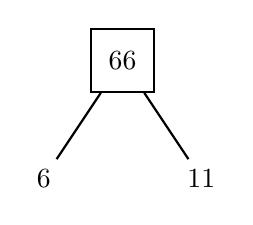
\begin{tikzpicture}[
    thick,
    level distance=1.5cm,
    sibling distance=2cm,
    edge from parent/.style={draw, -},
    % Composite style: Stays in Glaucous to differentiate from primes
    composite/.style={
        rectangle,
        draw=black,
        fill=white,
        minimum size=8mm,
        },
    ]
    \node [composite] {66}
    child {node {6}
    }
    child {node {11}};

\end{tikzpicture}
\xmalt{A partial factorization tree for the number 66. The top node is 66, which branches into 6 and 11.}
\end{center}


\item[Step 2] \textbf{Evaluate Each Factor}: \ Since 11 is prime it's circled.  The number 6 is not prime, so the process is repeated
in the next step.  

\begin{center}
\begin{tikzpicture}[
    thick,
    level distance=1.5cm,
    sibling distance=2cm,
    edge from parent/.style={draw, -},
    % Prime style: Funky Olive with a thick border to make it pop
    prime/.style={
        circle,
        draw=funkyolive,
        fill=funkyolive!10,
        line width=1.5pt,
        minimum size=9mm
    },
    % Composite style: Stays in Glaucous to differentiate from primes
    composite/.style={
        rectangle,
        draw=black,
        fill=white,
        minimum size=8mm
        },
]

\node [composite] {66}
    child {node [composite] {6}
    }
    child {node [prime] {11}};

\end{tikzpicture}

\xmalt{A partial factorization tree for the number 66. The top node is 66, which branches into 6 and 11. The number 11 is circled since it's prime.}

\end{center}


\item[Step 3]  \textbf{Repeat the Process}:  \ We can write 6 as the product of 2 and 3.  Since both 2 and 3 are prime, they are circled
and the tree is now finished.


\begin{center}
\begin{tikzpicture}[
    thick,
    level distance=1.5cm,
    sibling distance=2cm,
    edge from parent/.style={draw, -},
    % Prime style: Funky Olive with a thick border to make it pop
    prime/.style={
        circle,
        draw=funkyolive,
        fill=funkyolive!10,
        line width=1.5pt,
        minimum size=9mm
    },
    % Composite style: Stays in Glaucous to differentiate from primes
    composite/.style={
        rectangle,
        draw=black,
        fill=white,
        minimum size=8mm
        },
]

\node [composite] {66}
    child {node [composite] {6}
        child {node [prime] {2}}
        child {node [prime] {3}}
    }
    child {node [prime] {11}};

\end{tikzpicture}

\xmalt{A factorization tree for the number 66. The top node is 66, which branches into 6 and 11. The number 11 is circled since it's prime. The number 6 branches further into 2 and 3, both of which are circled since they are prime.}
\end{center}


\item[Step 4] \textbf{Final Result}: \ The prime factorization of 66 is the product of all circled numbers in the tree.

\[ 66 = 2 \cdot 3 \cdot 11 \]

\end{description}


\end{explanation}

\end{example}

\begin{remark}
No matter which factors you choose to start with, your tree will always end with the same set of prime numbers.  In the figure below, there are two factorization
trees for 100.  One begins with the factors 10 and 10 and the other begins with 2 and 50, but they both result in the same prime factorization.

\begin{center}
\begin{tikzpicture}[
    thick,
    level distance=1.5cm,
    sibling distance=2.5cm,
    level 2/.style={sibling distance=1.5cm},
    edge from parent/.style={draw, -},
    prime/.style={
        circle,
        draw=funkyolive,
        fill=funkyolive!10,
        line width=1.5pt,
        minimum size=9mm
    },
    % Composite style: Stays in Glaucous to differentiate from primes
    composite/.style={
        rectangle,
        draw=black,
        fill=white,
        minimum size=8mm
    }
]
    % Left Tree: Balanced (10 x 10)
    \begin{scope}[shift={(-3.5,0)}]
        \node [composite] {100}
            child {node [composite] {10}
                child {node [prime] {2}}
                child {node [prime] {5}}
            }
            child {node [composite] {10}
                child {node [prime] {2}}
                child {node [prime] {5}}
            };
        \node at (0,-4.5) {$100 = 2 \cdot 2 \cdot 5 \cdot 5$};
    \end{scope}

    % Right Tree: Linear (2 x 50)
    \begin{scope}[shift={(3.5,0)}]
        \node [composite] {100}
            child {node [prime] {2}}
            child {node [composite] {50}
                child {node [prime] {2}}
                child {node [composite] {25}
                    child {node [prime] {5}}
                    child {node [prime] {5}}
                }
            };
        \node at (0,-6) {$100 = 2 \cdot 2 \cdot 5 \cdot 5$};
    \end{scope}
\end{tikzpicture}

\xmalt{Two factorization trees for the number 100 shown side-by-side. The left tree branches into two 10s, each branching into prime factors 2 and 5. The right tree branches into 2 and 50, then 50 branches into 2 and 25, then 25 branches into 5 and 5. Both trees show the final prime factorization 100 equals 2 times 2 times 5 times 5.}

\end{center}

\end{remark}



\begin{problem}
The factorization tree for the number 30 is given below.

\begin{center}
\begin{tikzpicture}[
    thick,
    level distance=1.5cm,
    sibling distance=2cm,
    edge from parent/.style={draw, -},
    % Prime style: Funky Olive with a thick border
    prime/.style={
        circle,
        draw=funkyolive,
        fill=funkyolive!10,
        line width=1.5pt,
        minimum size=9mm,
        font=\normalfont  % Removes the slanted font
    },
    % Composite style: Simple white boxes
    composite/.style={
        rectangle,
        draw=black,
        fill=white,
        minimum size=8mm,
        font=\normalfont
    }
]
\node [composite] {30}
    child {node [prime] {2}}
    child {
        node [composite] {15}
        child {node [prime] {3}}
        child {node [prime] {5}}
    };
\end{tikzpicture}
\xmalt{A factorization tree for the number 30. The top node is 30, which branches into 2 and 15. The number 2 is circled. The number 
15 branches further into 3 and 5, both of which are circled.}
\end{center}


Based on this tree, what is the prime factorization of $30$?

\begin{multipleChoice}
    \choice{$2 \cdot 15$}
    \choice[correct]{$2 \cdot 3 \cdot 5$}
    \choice{$2 \cdot 3 \cdot 10$}
    \choice{$2 \cdot 3 \cdot 5 \cdot 15$}
\end{multipleChoice}

\begin{feedback}
    To find the prime factorization, only multiply the numbers in the circles at the very ends of the branches. Composite numbers in boxes (like 15) are just stepping
    stones.
\end{feedback}
\end{problem}


\begin{problem}
The factorization tree for the number 140 is given below.

\begin{center}
\begin{tikzpicture}[
    thick,
    level distance=1.5cm,
    sibling distance=2.5cm,
    edge from parent/.style={draw, -},
    % Prime style: Funky Olive with a thick border
    prime/.style={
        circle,
        draw=funkyolive,
        fill=funkyolive!10,
        line width=1.5pt,
        minimum size=9mm,
        font=\normalfont  % Removes the slanted font
    },
    % Composite style: Simple white boxes
    composite/.style={
        rectangle,
        draw=black,
        fill=white,
        minimum size=8mm,
        font=\normalfont
    }
]
\node [composite] {140}
    child {
        node [composite] {20}
        child {
            node [composite] {4}
            child {node [prime] {2}}
            child {node [prime] {2}}
        }
        child {node [prime] {5}}
    }
    child {node [prime] {7}};
\end{tikzpicture}
\xmalt{A factorization tree for the number 140. The top node is 140, branching into 20 and 7. The 20 branches into 4 and 5, and the 4 branches into two circled 2s. The prime numbers 2, 2, 5, and 7 are circled.}
\end{center}

Based on this tree, what is the prime factorization of $140$?

\begin{multipleChoice}
    \choice{$2 \cdot 2 \cdot 35$}
    \choice{$4 \cdot 5 \cdot 7$}
    \choice[correct]{$2 \cdot 2 \cdot 5 \cdot 7$}
    \choice{$2 \cdot 5 \cdot 7 \cdot 20$}
\end{multipleChoice}


\end{problem}


\begin{problem} Find the prime factorization of $42$.

  \begin{multipleChoice}
    \choice{$6 \cdot 7$}
    \choice{$2 \cdot 21$}
    \choice[correct]{$2 \cdot 3 \cdot 7$}
    \choice{$2 \cdot 3 \cdot 3 \cdot 7$}
  \end{multipleChoice}

  \begin{hint}
    Think of a pair of factors for $42$. For example, $42 = 6 \cdot 7$. Since $7$ is prime, you only need to factor $6$.
  \end{hint}
\end{problem}


\begin{problem}
  Find the prime factorization of $120.$

  \begin{multipleChoice}
    \choice{$10 \cdot 12$}
    \choice{$2 \cdot 2 \cdot 3 \cdot 10$}
    \choice[correct]{$2 \cdot 2 \cdot 2 \cdot 3 \cdot 5$}
    \choice{$2 \cdot 3 \cdot 4 \cdot 5$}
  \end{multipleChoice}


\end{problem}

\section*{Extra Insight:  The Power of Prime Numbers}

Did you know that \textbf{prime numbers} keep your online data safe from hackers?  Secure messages and accounts are locked by 
a giant composite number and the key is its prime factorization.  One way this is done is through a process called \textbf{RSA Encryption}.  
To create the lock, a computer picks two very large prime numbers and multiplies them together to get an enormous composite number.  
A computer can multiply two very large prime numbers in less than a second to create the composite number, but finding its prime 
factorization is very difficult!  It would take the fastest supercomputer billions of years.  Since its nearly impossible for hackers 
to find the key (the prime factorization), your accounts and messages stay locked and your information remains private!

This whole process depends on knowing two very large prime numbers. The largest known prime number was discovered in 2024 and is 
over 41 million digits long! People use a network of thousands of computers (called GIMPS) to hunt for these massive prime numbers 
nd there is even a cash prize for the person who finds the next one.





\end{document}